%
% dtf.tex -- Idee mit DFT
%
\section{Übertragung mit Hilfe der Diskrten Fourientransformation
\label{reedsolomon:section:dtf}}
\rhead{Umwandlung mit DTF}
Um die Polynominterpolation zu umgehen, gehen wir nun über in die Fourietransformation.
Dies wird weder eine Erklärung der Forientransorfmation, noch ein genauer gebrauch für den Reed-Solomon-Code. 
Dieser Abschnitt zeigt nur wie die Fourietransformation auf Fehler reagiert.
Das ganze zeigen wir mit einem Beispiel einer Übertragung von Zahlen mit Hilfe der Fourietransformation.

\subsection{Diskrete Fourietransformation Zusamenhang
\label{reedsolomon:subsection:dtfzusamenhang}}
Mit hilfe der Fourietransformation werden die \textcolor{blue}{blauen Datenpunkte} transformiert,
zu den \textcolor{darkgreen}{grünen Übertragungspunkten}. 
Durch eine Rücktransformation könnnen die \textcolor{blue}{blauen Datenpunkte} wieder rekonstruiert werden.

\subsubsection{Beispiel einer Übertragung
\label{reedsolomon:subsection:Übertragungsabfolge}}
Der Auftrag ist nun 64 Daten zu übertragen und nach 32 Fehler abzusicheren,
16 Fehler erkennen und rekonstruieren.

Dieser Auftrag soll mittels Fouriertransformation bewerkstelligt werden.
In der Abbildung \ref{reedsolomon:subsection:Übertragungsabfolge} sieht man dies Schritt für Schritt,
und hier werden die einzelne Schritte erklärt:
\begin{enumerate}[(1)]
 \item Das Signal hat 64 die Daten $k$, hier zufällige Zahlen, welche übertragen werden sollen. 
 Zusätzlich soll nach 16 Fehler $t$, die rekonstruierbar sind abgesichert werden.
 Das macht dann insgesamt $k + 2t = 
 64 +2 \cdot 16= 96$ Übertragungszahlen.
 (siehe Abschnitt \externaldocument{papers/reedsolomon/idee}\ref{reedsolomon:section:Fehlerkorrekturstellen})
 Die 32 Fehlerkorrekturstellen werden als Nullzahlen Übertragen.
 \item Nun werden mittels der diskreten Fourietransformation diese 96 codiert, transformiert.
 Das heisst alle Informationen ist in alle Zahlenvorhanden, auch die Fehlerkorrekturstellen Nullzahlen.
 \item Nun kommen drei Fehler dazu an den Übertragungsstellen 7, 21 und 75.
 Die Fehler können auf den ganzen 96 Übertragungswerten liegen, wie die 75 zeigt.
Zu Beachten ist auch noch, dass der Fehler um das 20- bis 150-Fache kleiner ist.Die Fehlerskala ist rechts.
 \item Dieses wird nun Empfangen, man kann keine Fehler erkennen, da diese soviel kleiner sind.
 Für das Decodieren wird die Inverse Fourietransformation angewendet, und alle Fehler werden mittransformiert.
 \item Nun sieht man die Fehler im decodierten Signal in den Übertragungszahlen. 
 Von den Übertragungsstellen 64 bis 96 erkennt man, das diese nicht mehr Null sind.
 \item Diese Fehlerkorrekturstellen 64 bis 96, dies definieren wir als Syndrom.
 In diesem Syndrom ist die Fehlerinformation gespeichert und muss nur noch transformiert werden.
 \item Hier sieht man genau wo die Fehler stattgefunden haben. 
 Leider nicht mehr mit der Qualtiätt der Ursprünglichen Fehler, sie sind nur noch 0.6 oder 0.4 gross.
 Obwohl der Fehler um das 20Fache kleiner ist erkennt man im Locator die Fehlerstellen wieder.
 \end{enumerate}
 Nun haben wir mit Hilfe der Fourietransformation die 3 Fehlerstellen durch das Syndrom lokalisiert, 
 jetzt gilt es nur noch diese zu korrigieren und wir haben unser originales Signal wieder.
\begin{figure}
	\centering
	\resizebox{1.1\textwidth}{!}{
	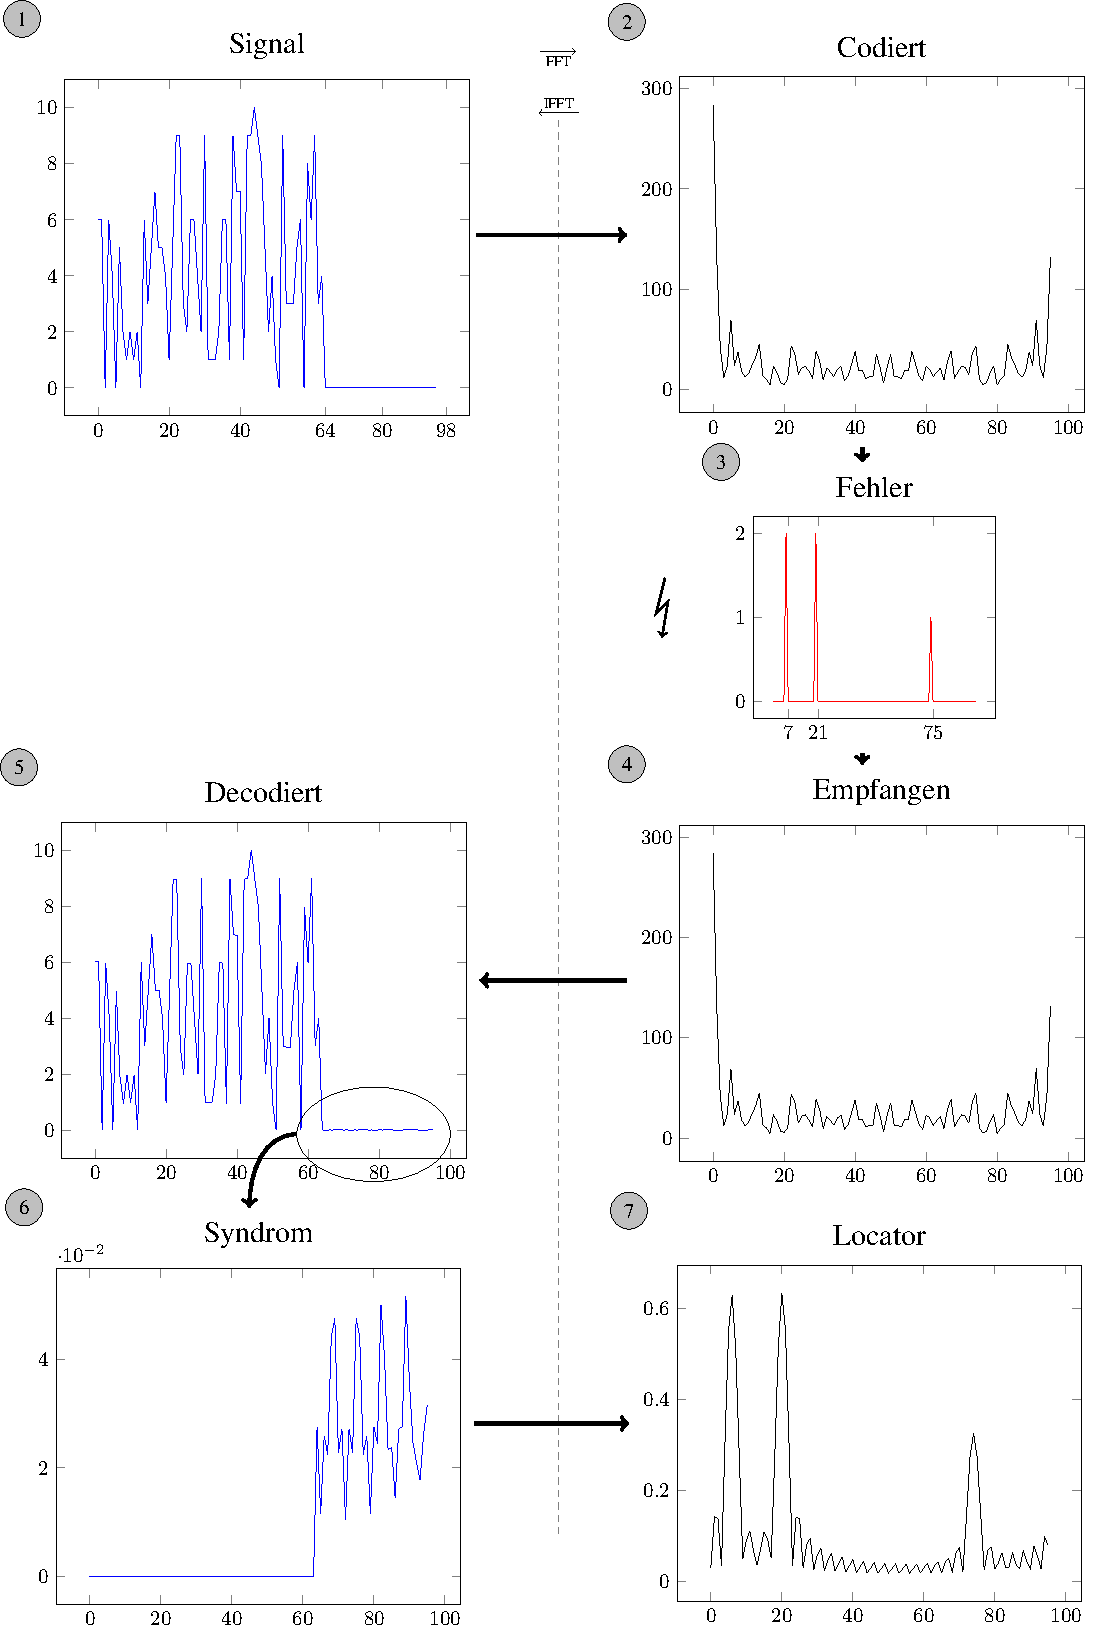
\includegraphics[width=\textwidth]{papers/reedsolomon/figures/plotfft}
    %
\begin{tikzpicture}[]

	%---------------------------------------------------------------
	%Knote
	\matrix(m) [draw = none, column sep=25mm, row sep=2mm]{

		\node(signal)  []    {
		\begin{tikzpicture}
			\begin{axis}
				[title = {\Large {Signal}}, 
				xtick={0,20,40,64,80,98}]
				\addplot[blue] table[col sep=comma] {tikz/signal.txt};
			\end{axis}
		\end{tikzpicture}}; &
		
		\node(codiert) []    {
		\begin{tikzpicture}[]
			\begin{axis}[ title = {\Large {Codiert \space + \space Fehler}},
				xtick={0,40,60,100}, axis y line*=left]
				\addplot[green] table[col sep=comma] {tikz/codiert.txt};
			\end{axis}
			\begin{axis}[xtick={7,21,75}, axis y line*=right]
					\addplot[red] table[col sep=comma] {tikz/fehler.txt};
			\end{axis}
		\end{tikzpicture}}; \\
		
		\node(decodiert) []    {
		\begin{tikzpicture}
			\begin{axis}[title = {\Large {Decodiert}}]
				\addplot[blue] table[col sep=comma] {tikz/decodiert.txt};
			\end{axis}
		\end{tikzpicture}}; &
	
		\node(empfangen) []    {
		\begin{tikzpicture}
			\begin{axis}[title = {\Large {Empfangen}}]
				\addplot[green] table[col sep=comma] {tikz/empfangen.txt};
			\end{axis}
		\end{tikzpicture}};\\
	
		\node(syndrom) []   {
		\begin{tikzpicture}
			\begin{axis}[title = {\Large {Syndrom}}]
				\addplot[black] table[col sep=comma] {tikz/syndrom.txt};
			\end{axis}
		\end{tikzpicture}}; &
	
		\node(locator) []    {
		\begin{tikzpicture}
			\begin{axis}[title = {\Large {Locator}}]
				\addplot[gray] table[col sep=comma] {tikz/locator.txt};
			\end{axis}
		\end{tikzpicture}};\\
	};
	%-------------------------------------------------------------
		%FFT & IFFT deskription
	
	\draw[thin,gray,dashed] (0,9) to (0,-9);
	\node(IFFT)  [scale=0.9]  at (0,9.3)   {IFFT};
	\draw[stealth-](IFFT.south west)--(IFFT.south east);
	\node(FFT)  [scale=0.9, above of=IFFT]    {FFT};
	\draw[-stealth](FFT.north west)--(FFT.north east);
	
	\draw[thick, ->,] (codiert)++(-1,0) +(0.05,0.5) -- +(-0.1,-0.1) -- +(0.1,0.1) -- +(0,-0.5);
	%Arrows
	\draw[thick, ->] (signal.east) to (codiert.west);
	\draw[thick, ->] (codiert.south) to (empfangen.north);
	\draw[thick, ->] (empfangen.west) to (decodiert.east);
	\draw[thick, ->] (syndrom.east) to (locator.west);
	\draw[thick](decodiert.south east)++(-1.8,1)  ellipse (1.3cm and 0.8cm) ++(-1.3,0) coordinate(zoom) ;
	\draw[thick, ->] (zoom) to[out=180, in=90] (syndrom.north);
	
	%item
	\node[circle, draw, fill =lightgray] at (signal.north west) {1};
	\node[circle, draw, fill =lightgray] at (codiert.north west) {2+3};
	\node[circle, draw, fill =lightgray] at (empfangen.north west) {4};
	\node[circle, draw, fill =lightgray] at (decodiert.north west) {5};
	\node[circle, draw, fill =lightgray] at (syndrom.north west) {6};
	\node[circle, draw, fill =lightgray] at (locator.north west) {7};
\end{tikzpicture}	
	}
	\caption{Übertragungsabfolge \ref{reedsolomon:subsection:Übertragungsabfolge}}
	\label{fig:sendorder}
\end{figure}

Nun zur Definition der Diskrete Fourietransformation, diese ist definiert als
 \begin{equation}
	\hat{c}_{k} 
	= \frac{1}{N} \sum_{n=0}^{N-1}
	{f}_n \cdot e^{-\frac{2\pi j}{N} \cdot kn}.
	,\label{reedsolomon:DFT}
 \end{equation}
 Wenn man nun 
 \begin{equation}
	w =
	e^{-\frac{2\pi j}{N} k}
	\label{reedsolomon:DFT_summand}
 \end{equation}
 ersetzte, und $N$ konstantbleibt, erhält man
 \begin{equation}
	\hat{c}_{k}=
	\frac{1}{N}( {f}_0 w^0 + {f}_1 w^1 + {f}_2 w^2 + \dots + {f}_{N-1} w^N)
	\label{reedsolomon:DFT_polynom}
 \end{equation}
 was überaust ähnlich zu unserem Polynomidee ist.
Die Polynominterpolation und die Fourietransformation rechnen beide mit reelen Zahlen.
Wenn die Fehlerabweichung sehr sehr klein ist, erkennt man diese irgendwann nicht mehr.
Zusätzlich muss mann immer Grenzen bestimmen auf wieviel Stellen gerechnet wird und wie die Fehler erkannt werden im Locator.
Deshalb haben Mathematiker einen neuen Körper gesucht und ihn in der Endlichkeit gefunden,
dies wird nun im nächsten Abschnitt genauer erklärt.

